%% Erl�uterungen zu den Befehlen erfolgen unter
%% diesem Beispiel.
\documentclass[DIV12]{scrartcl}
%\documentclass{article}
\usepackage[latin1]{inputenc}
%\usepackage[T1]{fontenc}
%\usepackage[ngerman]{babel}
\usepackage{amsmath}
\usepackage{makeidx}
\usepackage{hyperref}
\usepackage{fullpage}
\usepackage{listings}
\usepackage{color}
\usepackage{tikz}
\usepackage{listings}
\definecolor{gray}{gray}{0.9}
\usepackage{graphicx}
\usetikzlibrary{snakes}
\newcommand{\photoss}{\textsc{Photoss}}
\newcommand{\pjob}{\textsc{Pjob}}
\newcommand{\matlab}{\textsc{Matlab}}
\newcommand{\pho}{.pho}
\newcommand{\pscript}{.pscript}

\title{The PJOB file format\\Version 1.0}
\author{Dipl.-Inf. Nicolas Luck\\Dipl.-Phys. Matthias Westh�user\\Dipl.-Phys. Christian Remmersmann\\
		High Frequency Institute at the TU Dortmund}
\date{\today}

\begin{document}
 
\maketitle
\tableofcontents
\newpage

%\twocolumn



\section{Introduction}
\pjob\ is a file format implemented by the simulation tool \photoss\footnote{\url{http://www.photoss.de}}.
It was introduced to make the creation and sharing of complex simulation scenarios easier for the user.
A \pjob\ file incorporates all data necessary to run a complex job.
Depending on the actual simulation scenario this may be several \pho\ files, \matlab\ files, \pscript\ files
or some user defined data structures.

When running a \pjob\ file \photoss\ writes the simulation results into the executed \pjob\ file.
Already existing results are preserved so a \pjob\ file saves the history of all executions of a job.
A \pjob\ file uses XML files to determine what parameters may be provided when executing the job,
what results are created and in which files these results are written.





\section{Structure}
\pjob\ files are archives containing a particular file structure as depicted in figure \ref{filestructure}.
\begin{figure}[h!]
%\centering
\caption{File structure of a \pjob\ file. \textbf{Bold} entries represent directories.}
\label{filestructure}
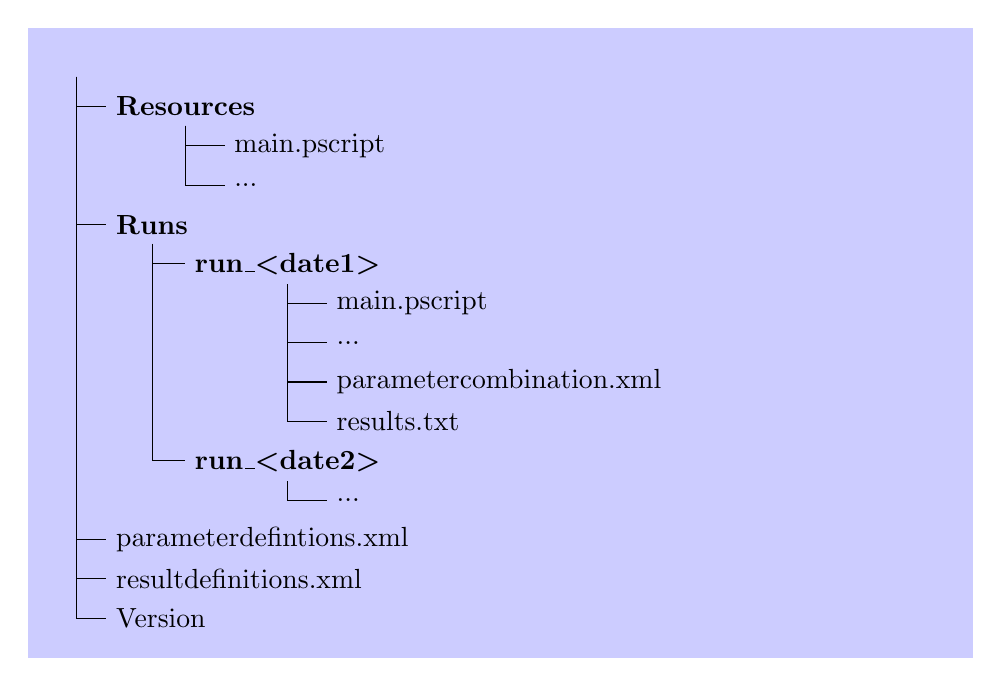
\begin{tikzpicture}
\fill[blue!20] (0,0) rectangle (12cm,-8cm);
\draw (0.5,-0.5) node[anchor=west](root) {\\};
	\draw (1,-1) node[anchor=west,font=\bfseries](Res) {Resources};
		\draw (2.5,-1.5) node[anchor=west](main) {main.pscript};
		\draw (2.5,-2) node[anchor=west] (ResDots){...};
	\draw (1,-2.5) node[anchor=west,font=\bfseries] (Runs) {Runs};
		\draw (2,-3) node[anchor=west,font=\bfseries] (Run1) {run\_\textless date1\textgreater};
			\draw (3.8,-3.5) node[anchor=west](Run1Main) {main.pscript};
			\draw (3.8,-4) node[anchor=west] (Run1Dots) {...};
			\draw (3.8,-4.5) node[anchor=west](Run1Params) {parametercombination.xml};
			\draw (3.8,-5) node[anchor=west](Run1Results) {results.txt};
		\draw (2,-5.5) node[anchor=west,font=\bfseries] (Run2) {run\_\textless date2\textgreater};
			\draw (3.8,-6) node[anchor=west] (Run2Dots) {...};
	\draw (1,-6.5) node[anchor=west] (Parameterdefinitions) {parameterdefintions.xml};
	\draw (1,-7) node[anchor=west] (Resultdefinitions) {resultdefinitions.xml};
	\draw (1,-7.5) node[anchor=west] (Version) {Version};

\draw (root.south) |- (Res.west);
\draw (root.south) |- (Runs.west);
\draw (root.south) |- (Parameterdefinitions.west);
\draw (root.south) |- (Resultdefinitions.west);
\draw (root.south) |- (Version.west);
\draw (Res.south) |- (main.west);
\draw (Res.south) |- (ResDots.west);
\draw (Runs.south) |- (Run1.west);
\draw (Runs.south) |- (Run2.west);
\draw (Run1.south) |- (Run1Dots.west);
\draw (Run1.south) |- (Run1Main.west);
\draw (Run1.south) |- (Run1Params.west);
\draw (Run1.south) |- (Run1Results.west);
\draw (Run2.south) |- (Run2Dots.west);
\end{tikzpicture}
\end{figure}


The following entries are mandatory:
\begin{itemize}
\item Directory \textit{Resources} containing a file \textit{main.pscript}
\item Directory \textit{Runs} (may be empty)
\item Files \textit{parameterdefintions.xml}, \textit{resultdefinitions.xml} and \textit{Version}
\end{itemize}
The directory \textit{Resources} may contain any number of files or directories of any depth.
\textit{Resources/main.pscript} must be a valid \textsc{PScript} file.
For every (already completed) execution of the job there is a subdirectory in the \textit{Run} directory.
These subdirectories are named \textit{run\_} plus the date of the execution
in the format \textit{YYYYMMDD\_hhmm} (so that lexical sorting makes it easy to find the latest run).

File \textit{Version} contains the \pjob\ file's version as string.
So for the first version this is \textit{"1.0"}. Will be different in future versions of \pjob\ files.

\subsection{Underlying archive format}
\pjob\ files use a self-made binary archive format to concatenate the files contained in a \pjob\ file.
The first 21 bytes are occupied by the file header.
It starts with the 9 byte string \texttt{PJobFile\textbackslash n}
followed by the file's version number represented as a 4 byte little endian integer (TODO: signed or unsigned?).
The header's third and last field is a 8 byte little endian long integer (TODO: signed or unsigned?)
that tells the files last modification date in seconds since the Unix Epoch (00:00:00 UTC on 1 January 1970).

The file's content consists of chunks,
one for every file that was archived in it.
Each chunk itself consists of a chunk header and its content (the file content).
The chunk header's first field is a newline terminated string that represents the filename
associated with this chunk,
including its relative (to this archive), forward slash (\texttt{/})
seperated file path (for example \texttt{Resources/main.pscript}).
The filename is followed by the file's last modification date as a 8 byte little endian long integer,
again representing the number of seconds since the Unix Epoch.
Third and last chunk header field is a 4 byte little endian integer representing
the chunk's body's size in bytes.
This is directly followed by the body that is the file's zlib compressed content.

\begin{figure}[h!]
\caption{\pjob's underlying binary format.}
\label{binary_format}
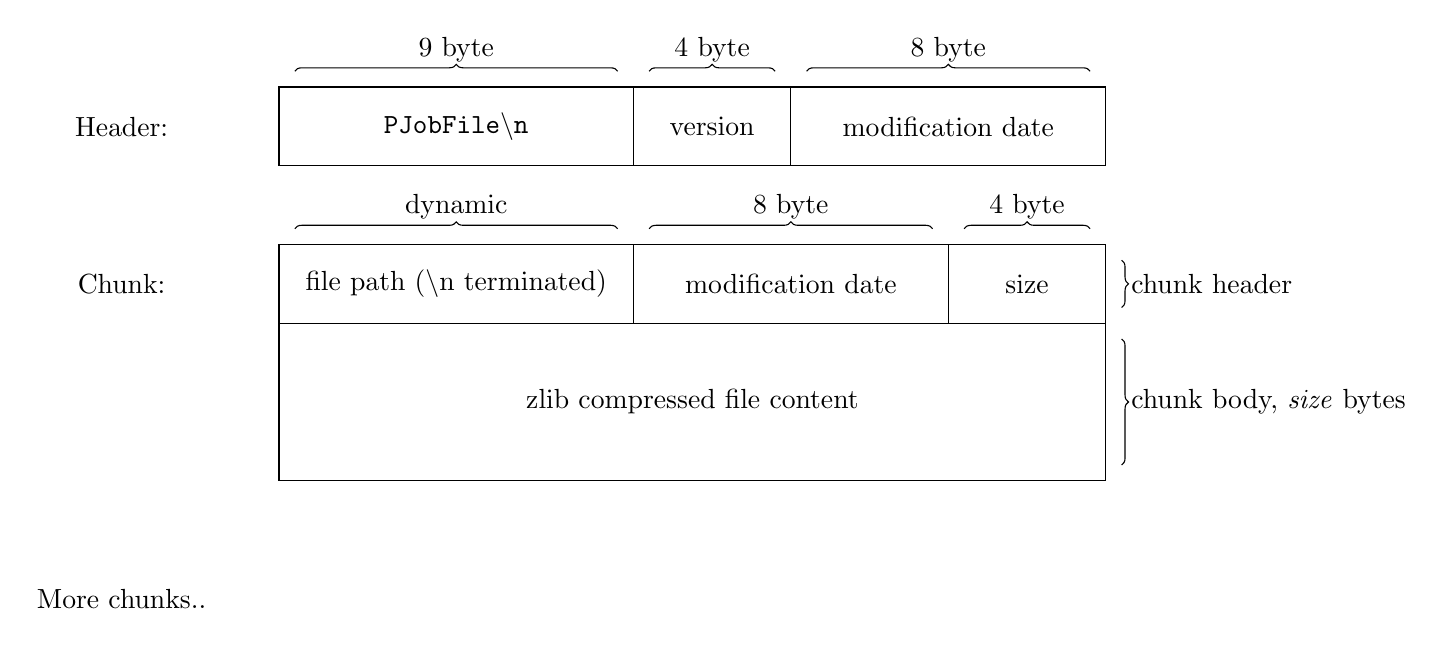
\begin{tikzpicture}
	\draw (-2,-0.5) node {Header:};
	\draw (0,0) rectangle (4.5,-1) rectangle (6.5,0) rectangle (10.5,-1);
	\draw (2.25, -0.5) node {\texttt{PJobFile\textbackslash n}}
	      (5.5, -0.5) node {version}
	      (8.5, -0.5) node {modification date};
	
    \draw[snake=brace] (0.2,0.2) -- node[above]{9 byte} (4.3,0.2)
                       (4.7,0.2) -- node[above]{4 byte} (6.3,0.2)
                       (6.7,0.2) -- node[above]{8 byte} (10.3,0.2);

    \draw (-2,-2.5) node {Chunk:};
    \draw (0,-2) rectangle (4.5,-3) rectangle (8.5,-2) rectangle (10.5,-3) rectangle (0,-5);
	\draw (2.25, -2.5) node {file path (\textbackslash n terminated)}
	      (6.5, -2.5) node {modification date}
	      (9.5, -2.5) node {size}
	      (5.25, -4) node {zlib compressed file content};
	
	\draw[snake=brace] (0.2,-1.8) -- node[above]{dynamic} (4.3,-1.8)
                       (4.7,-1.8) -- node[above]{8 byte} (8.3,-1.8)
                       (8.7,-1.8) -- node[above]{4 byte} (10.3,-1.8)
                       (10.7,-2.2) -- node[right]{chunk header} (10.7,-2.8)
                       (10.7,-3.2) -- node[right]{chunk body, \textit{size} bytes} (10.7,-4.8);

    \draw (-2,-6.5) node {More chunks..};
\end{tikzpicture}
\end{figure}

This format makes it easy to add files to the archive,
chunks can be appended at the end of the file.
There is no sorting required.
The tree-like file structure is based on the file names, which also include the path
and therefore the directory.
One (negligible) drawback is that there is no way to have an empty directory.
The file's contents can be scanned by hopping from chunk header to chunk header,
omitting the content.

\subsection{Parameters}
A \pjob\ file may declare parameters that can be assigned values to when executing the job with \photoss.
Once declared these parameteres will be available in the main.pscript's context,
that is the \pjob's script may assume that variables with the parameter's names
have been set before executing the main.pscript.
Furthermore the parameter's values are checked to be within the specified boundaries.

The file \textit{parameterdefinitions.xml} defines which parameters may be provided when executing the job.
This must be consistent with the code in \textit{main.pscript},
i.e. parameters needed by the script must be declared here.
For every parameter a name and a default value has to be provided,
a minimum or maximum value can be provided.
A \textit{parameterdefinitions.xml} file may look like this:
\lstset{basicstyle=\color{black},basicstyle=\tiny, backgroundcolor=\color{gray}}
\begin{lstlisting}
<parameterdefinitions>
	<parameter>
		<name>length</name>
		<defaultValue>100</defaultValue>
	</parameter>
	<parameter>
		<name>power</name>
		<unit>dBm</unit>
		<defaultValue>5</defaultValue>
		<min>1</min>
		<max>15</max>
	</parameter>
</parameterdefinitions>
\end{lstlisting}
A XML Schema Definition for this XML file is provided in the appendix.

When executed a \textit{parametercombination.xml} file is saved in the run directory.
This file contains the information for which parameter values the job was executed.
It is either constructed by \photoss\ according to the default values
provided with the \textit{parameterdefinitions.xml}
or it was passed by the user as an argument in order to run the job with parameter values
differing from the default values.

A \textit{parametercombination.xml} may look like this:
\begin{lstlisting}
<parametercombination>
	<parameter>
		<name>length</name>
		<value>50</value>
	</parameter>
	<parameter>
		<name>power</name>
		<variation>
			<min>3</min>
			<max>7</max>
			<step>1</step>
		</variation>
	</parameter>
</parametercombination>
\end{lstlisting}
Again a XML Schema Definition is provided in the appendix.

On execution parameters are made available to the script.
For every parameter defined in \textit{parameterdefinitions.xml}
the global Property
\begin{lstlisting}
Application.parameters
\end{lstlisting}
will have a property named as the corresponding parameter.
These properties have subproperties \textit{isVariation()}
and either \textit{value} or \textit{min}, \textit{max}, \textit{step} and \textit{values}.
So a \textit{main.pscript} according to the example stated above may look like this:
\lstset{language=Java}
\begin{lstlisting}
if(Application.parameters.length.isVariation()){
	for(var i in Application.parameters.length.values)
		...
}else{
	var length = Application.parameters.length.value;
}
\end{lstlisting}



\subsection{Results}
All files created on execution reside in the run directory.
Which files are created depends on the code contained in the file \textit{Resources/main.pscript}.
In order to be able to access a job's results without having to know its implementation
the file \textit{resultdefinitions.xml} declares which files contain results
and what format they use.
As of version 1.0 the only supported format is the CSV format used by \photoss\
for its parameter variation result files.
A \textit{resultdefinitions.xml} declaring one result file which contains two results may look like this:
\lstset{language=XML}
\begin{lstlisting}
<resultdefinitions>
	<resultFile>
		<filename>Results.txt</filename>
		<format>PHOTOSS_CSV</format>
		<result>
			<name>EOP</name>
		</result>
		<result>
			<name>Q</name>
			<unit>dB</unit>
		</result>
	</resultFile>
</resultdefinitions>
\end{lstlisting}




\section{Execution of a \pjob\ file}
When running a \pjob\ file \photoss\ first extracts its contents to a temporary directory.
It then creates a new subdirectory under \textit{Runs}
named \textit{run\_} plus the current date and time
and copies all files and directories from \textit{Resources} to that newly created run directory.
\photoss\ changes its current working directory to that run directory and
executes the \textsc{PScript} file \textit{main.pscript}.
As described above parameters are therefore added to the \textsc{PScript} context before evaluating the script.
After the script has finished execution the temporary directory
(with the newly created run directory and the results therein)
is written back to the \pjob\ file.







\begin{appendix}
\section{XSDs}
\noindent
Schema for parameterdefinitions.xml:
\lstset{basicstyle=\color{black},basicstyle=\tiny, backgroundcolor=\color{gray}}
\lstset{tabsize=2}
\lstset{language=XML}
\lstinputlisting{parameterdefinitions.xsd}

\noindent
Schema for parametercombination.xml:
\lstset{basicstyle=\color{black},basicstyle=\tiny, backgroundcolor=\color{gray}}
\lstinputlisting{parametercombination.xsd}

\noindent
Schema for parameterdefinitions.xml:
\lstset{basicstyle=\color{black},basicstyle=\tiny, backgroundcolor=\color{gray}}
\lstinputlisting{resultdefinitions.xsd}
\end{appendix}
\end{document}






